\chapter{Evaluation and Comparison}
This chapter can be seen as the culmination of this dissertation. All the constraints have been described but what about the results? Do the counterpoints found by the solver equal those of Johann Joseph Fux? This is what this chapter will try to answer by comparing the species one by one.

The evaluations of the first four species will be simple analyzes of the differences and common points between the first counterpoint produced by the solver with the default values and the Fux counterpoint presented at the beginning of each species chapter. The analysis of the fifth species will be more advanced by tweaking the solver parameters to obtain more interesting counterpoints. A YouTube video is available \textbf{\href{https://youtu.be/9yB4OGr4Cgk}{here}}\parencite{EvalYT} to listen to the counterpoints presented in this chapter. The video follows the order of the following sections and includes a description with the time codes of each counterpoint.

Determining what a good counterpoint is is subjective and cultural. The following criticisms are therefore also subjective and cultural. It will be tried to make sociological objectivity and axiological neutrality\footnote{Axiological neutrality is a methodological posture proposed by the sociologist Max Weber. This consists of the researcher becoming aware of his own values during his scientific work, in order to reduce as much as possible the biases that his own value judgments could cause. \parencite{AxioNeut}}. It is thus good to note that these last are given by a man of Belgian culture appreciating Western music. Most people would say that Fux's counterpoints "look very baroque". It is therefore hoped that the counterpoints of the solver, presented below, will also be baroque. Moreover, the first four species are complicated to judge because with the absence of rhythm, an interesting melody will remain monotonous.

Let's not forget that the main goal is to observe if constraint programming can be useful in the field of music. Finally, these tests are performed with a version of the solver still under development (dated May 17, 2023). Some default values may have changed in the meantime during updates.

\section{Evaluation of the First Species}
\begin{figure}[h]
    \centering
    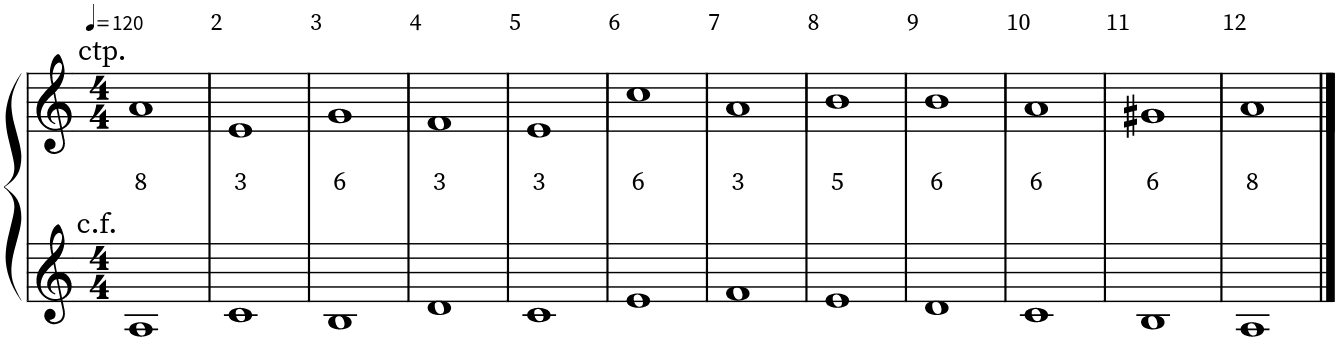
\includegraphics[height=\fhl]{Images/the_first_species.png}
    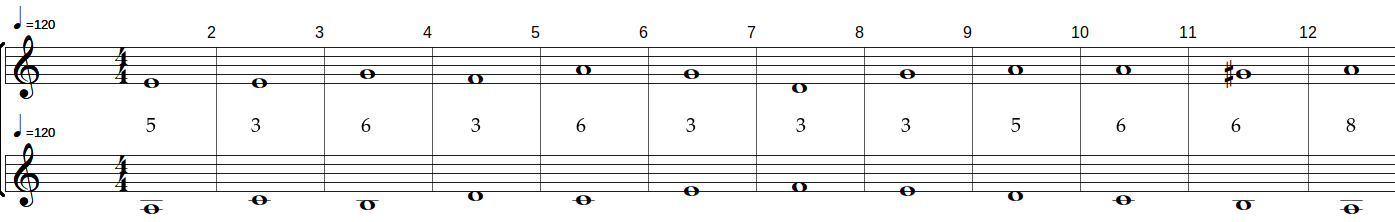
\includegraphics[width=\textwidth, height=\fhs]{Images/solver_1sp.png}
    \caption{\species{1} ctp. of Fux (above) vs. ctp. of the solver [0.132 s] (below).}
    \label{fig:eval_1sp}
\end{figure}
The two counterpoints (see figure \ref{fig:eval_1sp}\footnote{The solver solutions come from OpenMusic and have been stretched to better see the score lines.}) are globally very similar. A few differences are notable: the solver uses a fifth in \nth{1} measure and does not use a sixth leap from the \nth{5} to the \nth{6} measure. This makes sense because the sixth leap has a cost of 2. Moreover this leap is surprising on the part of Fux because it is not melodically very interesting. Between the \nth{9} and \nth{10} measures, a fifth and an oblique motion are used. They both have a cost of 1. It would be the same to not have a fifth, but a sixth and therefore have a direct motion between the \nth{9} and \nth{10} measure. It would make the end of the song more moving and interesting. Another point is that Fux uses five direct motions (motions supposed to be avoided) while the solver only uses one. This first example shows what the solver is capable of. It respects the rules well and never surprises because it is not aware of it. This point will be discussed further later.

\section{Evaluation of the Second Species}
\begin{figure}[h]
    \centering
    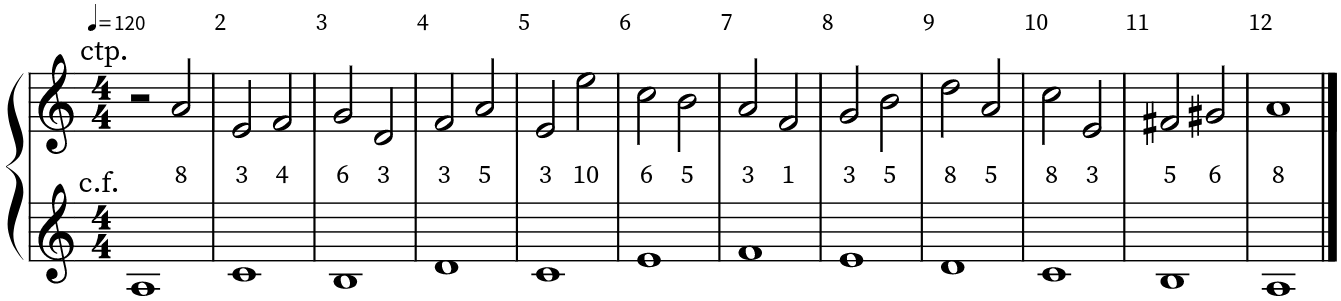
\includegraphics[height=\fh]{Images/the_second_species.png}
    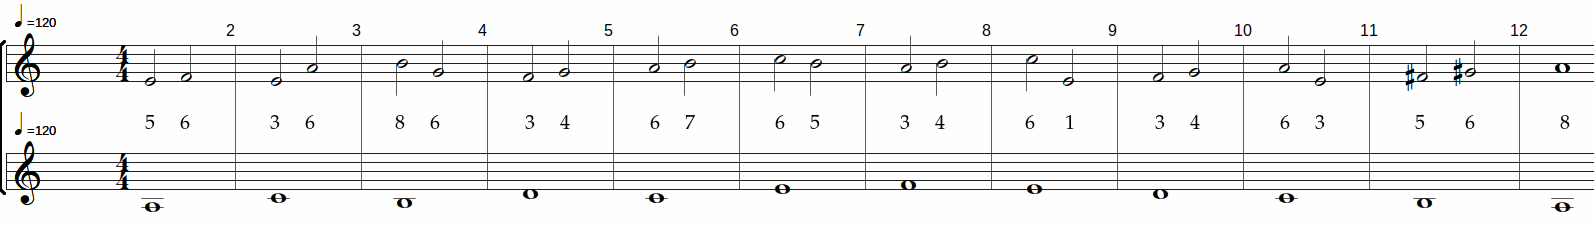
\includegraphics[width=\textwidth, height=\fhs]{Images/solver_2sp.png}
    \caption{\species{2} ctp. of Fux (above) vs. ctp. of the solver [26.849 s] (below).}
    \label{fig:eval_2sp}
\end{figure}
For the general feeling, the counterpoint of the solver is relatively of the same quality as that of Fux. Besides that, the solver's solution has a four-note motif from the arsis in the \nth{8} measure to the thesis in the \nth{10} measure ($E\to F\to G\to A$). This motif is repeated immediately raising the $F$ and the $G$ by a semitone. It sounds both strange and interesting but one can doubt that Fux would appreciate this melody.

A surprising point is the use that Fux makes of the big leaps between the notes in thesis and those in arsis. For example, he makes a fourth leap in the \nth{3} measure. According to rule \ref{rule:motion2nd}\footnote{Reminder: If the melodic interval of the counterpoint between the thesis and the arsis is larger than a third, then the motion is perceived based on the arsis note.}, the resulting motion is perceived from the note in arsis, i.e. the motion from the \nth{3} to the \nth{4} measure is considered direct (cost of 2) instead of contrary (no cost). This is typically the kind of behavior that does not occur with the solver.

Finally, one can notice that the search time for the answer is much higher than the previous one. This is a problem that particularly affects the second species and sometimes the fifth. This seems to come from rule \ref{rule:motion2nd} discussed just before. Indeed, the best solutions of the solver (in terms of costs) often use large leaps to have more contrary motions. It goes against stepwise melodies and therefore takes more time. As proof, if the cost of the motions is not taken into account, the solution is found in 0.2 seconds. Alternatively, a trade-off can be made by first adding branching from small values to the motions costs. Therefore, small costs for motions are calculated before other costs. The first solution found then deviates from the lowest possible cost but is found in 8 seconds. This is a fairly common optimization problem when the overall cost minimization is composed of inversely proportional costs.
% 8.537
% Now the most interesting point: Fux counterpoint cannot be generated by the solver. This is due to rule 42 which prevents the tenth bar from taking place. In fact, Fux doesn't quite do what it says. The constraint posed therefore does not correspond to the way in which he uses it. Indeed, Fux says "tatata". Outside the gap between the notes is still an octave. But on the other hand, it is true that during the process of composition, having arrived at the tenth bar, there is no other solution than to make a downward jump of six to allow a contrary movement towards the next straight. One would say that Fux should have predicted this to avoid this situation, the other would say that if he has no choice, then the rule is obeyed. The problem being that the solver is not in a linear composition process, it sees the whole thing at the same time. Rule 42 could be adapted so that leaps of minor sixths and octaves are also allowed when a perfect consonance is found in the next bar. But this chapter only aims to evaluate the current version of the solver, not to change it.

\section{Evaluation of the Third Species}
\begin{minipage}{0.60\textwidth}
    \begin{figure}[H]
        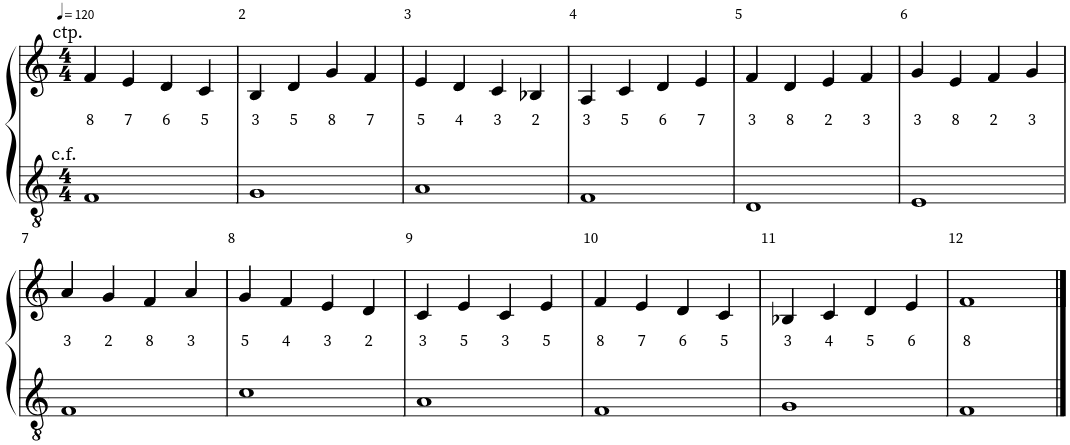
\includegraphics[width=1\textwidth, height=2.0in]{Images/complete_third_species_f.png}
        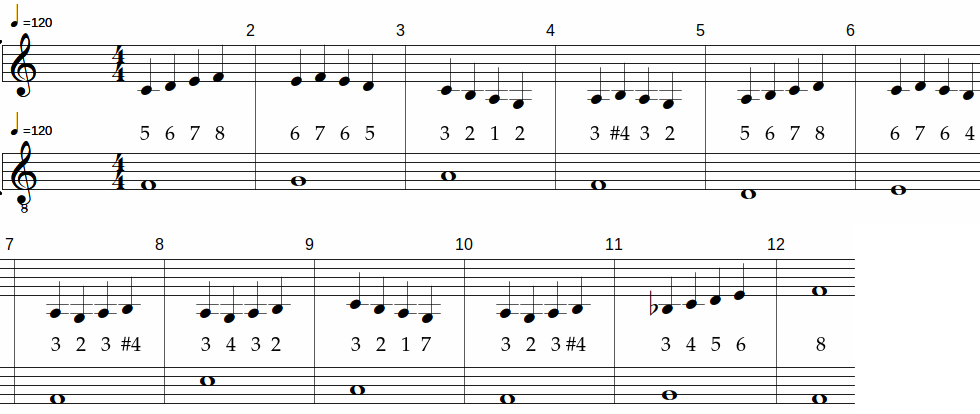
\includegraphics[width=1\textwidth, height=2.0in]{Images/solver_3sp.png}
        \caption{\species{3} ctp. of Fux (above) vs. ctp. of the solver [1.789 s] (below).}
        \label{fig:eval_3sp}
    \end{figure}
\end{minipage} \hfill
\begin{minipage}{0.38\textwidth}
    The solver's counterpoint is musically quite poor. Generally speaking, it is monotonous and rambling. Compared to that of Fux, it does not sound really baroque. The big negative point that emerges is the permanent use of stepwise melodic intervals. It is true that Fux is quite mysterious about the rules that make up a good melody and that he uses a lot of one-step intervals. However, "a lot" does not mean "all". This is a very important notion that will be developed later: adding to the solver this notion of compromise, of surprise, of "a little bit of that, a little bit of this", etc. Typically, a way to force a minimum of melodic skips has been added to the solver to counter this problem.
    Another way to solve that is to put no cost to the melodic intervals of third for example.\\
\end{minipage}

Also, the solver's counterpoint contains a redundant melody ($A\to G\to A\to B$) which isn't bad in itself but seems to be randomly repeated and unsatisfactory. Obviously, the solver has no notion concerning the repetition of a pattern. This is also a major point to improve so that the solver can generate more human melodies. This solver really lacks an adjustable notion of monotony.

A more detailed evaluation of the third species can be read in the article of \textcite{JIM}. It contributed to the improvement of this tool on the melodic level.

\section{Evaluation of the Fourth Species}
\begin{figure}[h]
    \centering
    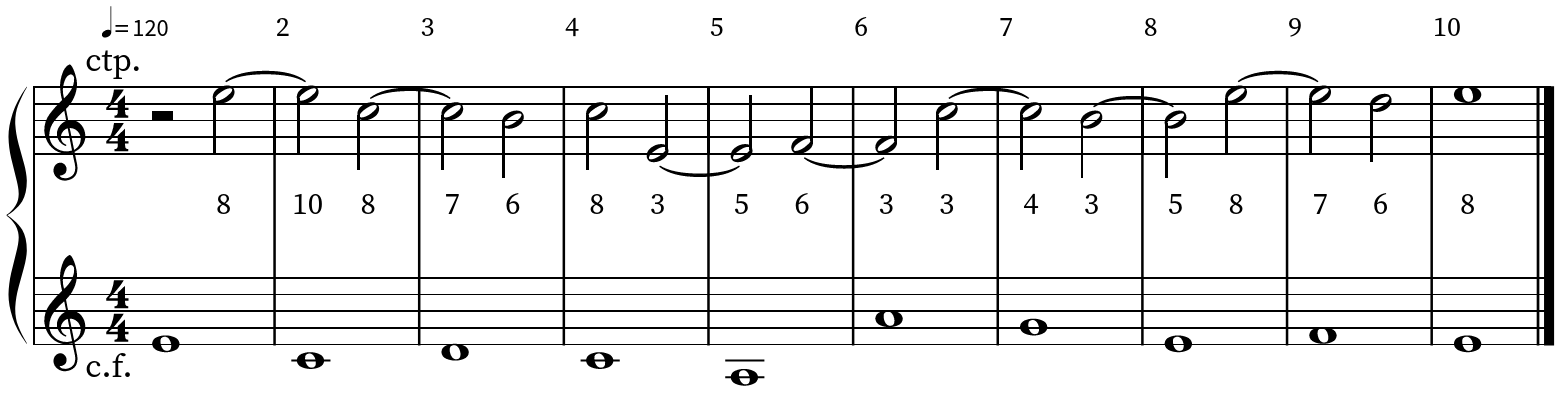
\includegraphics[height=\fhl]{Images/fux_4sp.png}
    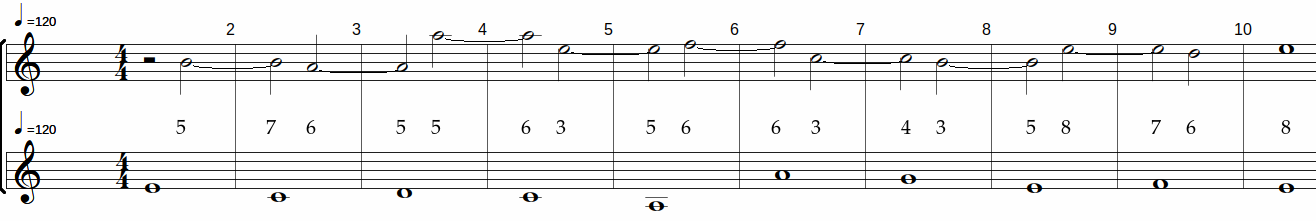
\includegraphics[width=\textwidth, height=\fhs]{Images/solver_4sp.png}
    \caption{\species{4} ctp. of Fux (above) vs. ctp. of the solver [0.012 s] (below).}
    \label{fig:eval_4sp}
\end{figure}
This example strongly highlights a defect of the solver: a poor melody. Indeed, the counterpoint is supposed to be composed of several melodies which, \emph{independently}, sound melodious and which, \emph{together}, sound harmonious. This horizontal vision of music is transcribed only through the fact that the counterpoint is generated from a counterpoint. But with Fux, no rule defines what the counterpoint should be as a consistent whole. In fact, his rules could be considered the "micro rules" of counterpoint. It would therefore be necessary for the solver to have "macro rules" defining the very structure of the counterpoint in its entirety.

In the \nth{5} and \nth{6} measure of Fux's counterpoint, the crossing between the two voices creates, for the time of three half notes ($F\to A\to C$), a rising melody by skips of third. This intertwining brings out an $F$ major chord giving that nostalgic feeling to the song. On the side of the solver, this opportunity is missed. But actually, the notes are "identical"\footnote{In terms of the diatonic scale.} from the second half of the \nth{4} measure. The only two real differences between those counterpoints are that the solver starts on a fifth and that it prefers an octave leap to the interruption of syncopations. This last point also shows that Fux exaggerates when he explains that syncope should be used "wherever possible"\parencite[p.89]{GaPEng}.

Although the generated counterpoint is average, it can allow a more or less experienced composer to find a good counterpoint by shifting a few notes by one octave. It's not perfect, but for a musician who likes to experiment, the solver gives him a good basis instantly that he can then exploit.

\section{Evaluation of the Fifth Species}
For this species, the analysis will be more advanced. First, the counterpoints will only be compared and secondly, a more compositional approach will be put forward. In section \ref{sec:5sp_comp}, the solver counterpoints are the first results obtained with the default values. In section \ref{sec:5sp_refine}, the solver will be used more intelligently to obtain a more interesting solution.
\subsection{Comparison}\label{sec:5sp_comp}
\begin{figure}[h]
    \centering
    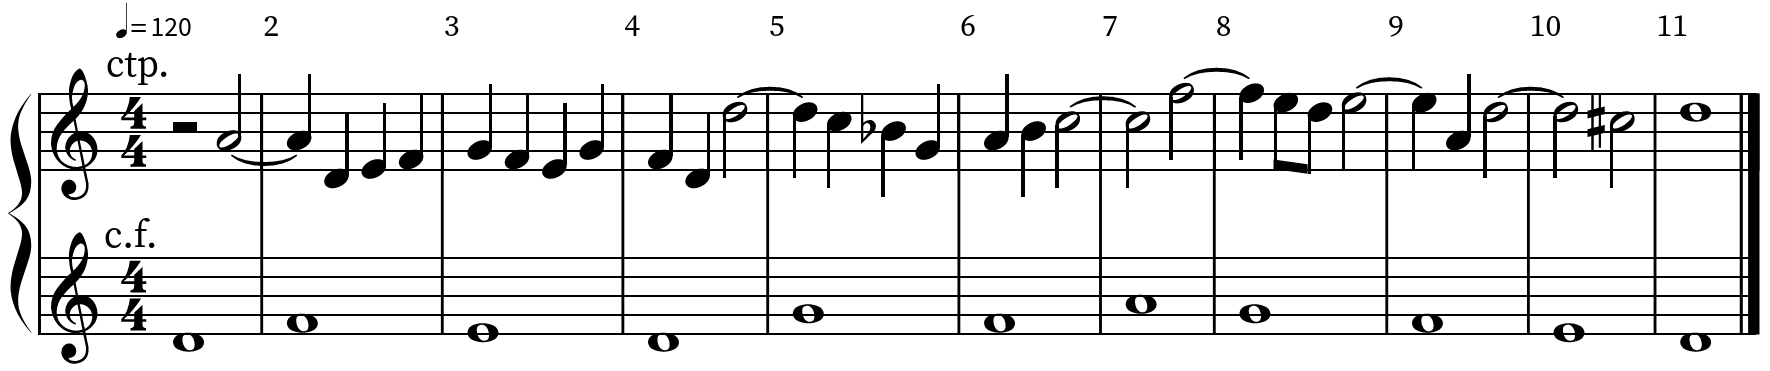
\includegraphics[height=\fhs]{Images/fux_5spA.png}
    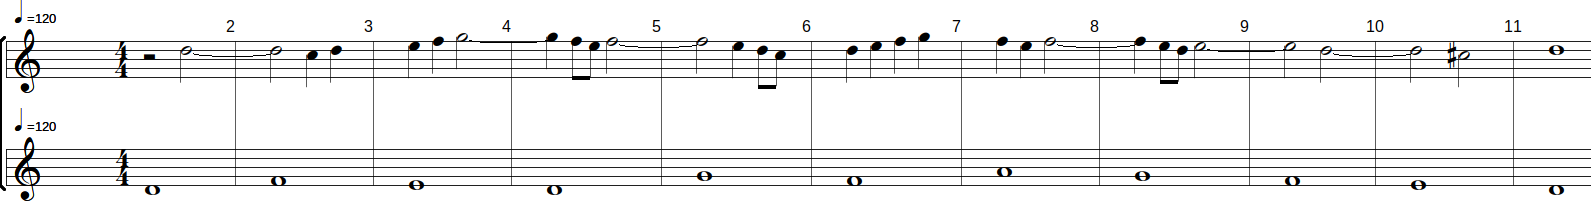
\includegraphics[width=\textwidth, height=1in]{Images/solver_5spA.png}
    \caption{\species{5} ctp. of Fux (above) vs. ctp. of the solver [0.174 s] (below).}
    \label{fig:eval_5spA}
\end{figure}

Whether it is the lower or upper counterpoint, those of Fux are clearly more baroque and are more melodious in general. Solvers' counterpoints aren't bad, but they're far from interesting. In figure \ref{fig:eval_5spA}, what Fux does in the \nth{4} and \nth{5} measure is the strong point of the work. The \nth{4} measure has a $D$ three times, which provides a pleasant rest before the repeat. He can afford this repetition because the $D$ is the tonic of the piece. The solver does not have this notion of rest and tension related to the underlying chord.

Also, the $B\flat$ in the \nth{5} measure adds a more nostalgic touch by suggesting a $G$ minor chord. This $B\flat$ is not repeated in the next measure, which is rather original. Again, it's these kinds of little details that make Fux's counterpoints sound better than solver ones. The problem is the same as with the third species, i.e. the melodies are too "stepwise". For information, the counterpoints in the lower part have been added in the appendix in figure \ref{fig:eval_5spB} and the criticisms are generally the same.

One topic that hasn't been covered so far is cost comparisons. Indeed, if we force the solver with the same notes as the Fux counterpoint, it is possible to know what its total cost is. This can give a good idea of how well Fux applies its own rules and whether the costs assigned by the solver are consistent in determining what is or is not a good counterpoint.

In this case, the solver's solution costs 14 while that of Fux costs 29. It makes sense that the solver finds solutions with a lower cost since that is the goal of its heuristic, unlike Fux. The cost discrepancy comes mainly from the common use of skips and leaps by Fux. This already costs 9 where the solver has none. This represents almost a third of the total cost. In fact, this way of optimizing costs is not entirely consistent with Fux's music. On the other hand, the melody should still be mainly stepwise. Maybe there is an alternative?


\subsection{Refinement}\label{sec:5sp_refine}
A point which was not specified in the previous section but which is important is the branching of the species array $S$.
Indeed, the rhythm of the species is the same for figure \ref{fig:eval_5spA}(below) and figure \ref{fig:eval_5spB}(below). It's not really a problem but the solver first randomly\footnote{The randomization is controlled and is done from a seed. Currently, the same seed is always used and there is no way to change it from the UI.} determines which species are going to be used before it starts determining the associated notes. Indeed, it is much harder for the solver to first find an inexpensive solution and then determine if a rhythm can be associated with it. However, it is expensive but not impossible. This further minimizes the cost.

Another point discussed above was the possibility of having more diversified solutions at the level of melodic intervals. Three options have therefore been added to the user interface.
\begin{itemize}
    \item \textit{Irreverence} artificially increases the minimum cost of the solution. This has two purposes: to prevent over-respecting solutions and/or to reduce the search time because the solver starts cost minimization with a higher lower bound.
    \item \textit{Minimum percentage of skips} forces the solver to use larger melodic intervals.
    \item \textit{Force joint contrary melody after skip} activates a rule\footnote{Coming from a work of \textcite{Bitsch}.} obliging a step melodic interval in the opposite direction after a skip.
\end{itemize}

\begin{multicols}{2}
    By using these options (see figure \ref{fig:irreverence_and_minskips}) and lowering the costs associated with the melodic intervals of thirds, fourths, and fifths by one notch, a more interesting solution can be generated.
    \begin{Figure}
        \centering
        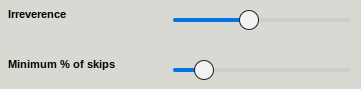
\includegraphics[scale=0.4]{Images/5sp_irreverence_and_minskips.png}
        \captionof{figure}{\textit{Irreverence} and \textit{Minimum percentage of skips} used for solution \ref{fig:solver_5sp_better}.}
        \label{fig:irreverence_and_minskips}
    \end{Figure}
\end{multicols}

\begin{figure}[h]
    \centering
    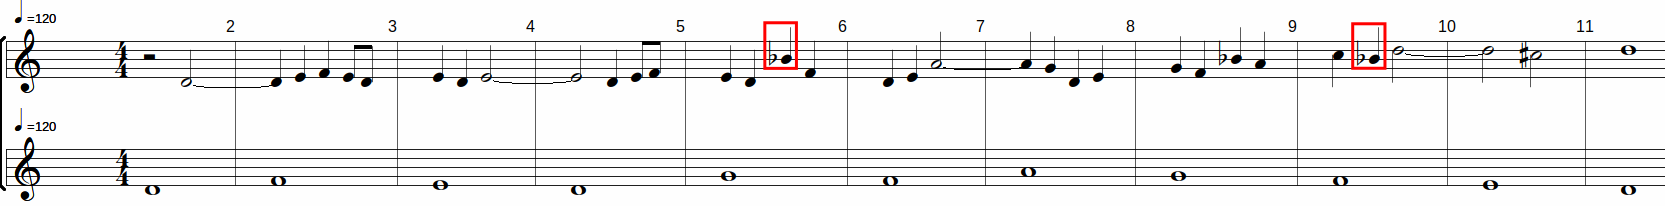
\includegraphics[width=\textwidth, height=1in]{Images/solver_5sp_bb.png}
    \caption{\species{5} refined counterpoint of the solver [2 min 58 s].}
    \label{fig:solver_5sp_better}
\end{figure}

This solution took nearly 3 minutes to be found, which is not huge but not negligible for a composer. Note that the notes boxed in \textcolor{red}{red} were changed to $B\flat$\footnote{These notes have only been transposed by one or two semitones to stay close to the original solution.} to try the solver in a more realistic context\footnote{Where a composer allows himself to change the few notes that bother him.}. With a few manipulations and tweaking, a good counterpoint is obtained in a few clicks and minutes. The solver shows that using it as a support tool can be very inspiring.

\section{Experimentation with the Fifth Species}\label{sec:5sp_experimentation}
On our side, as a "\textit{cantus firmus}", a more contemporary bass of 17 measures including chromatisms was tested. This example is presented at the end of the YouTube video\parencite{EvalYT} (at \href{https://youtu.be/9yB4OGr4Cgk?t=362}{6:02}) and shows the ability of the solver to adapt to "\textit{cantus firmus}" which are not at all classic. To be precise, the solver worked separately twice on this bassline with different preferences. In total, it generates a piece of 33 measures, in just over 3 minutes. The scores are available in the appendix in figure \ref{fig:exp_scores}.

We found that the result was stunning. This is clearly a sufficient starting point for at least one accompaniment in a piece of music. Indeed, it shows that even though the solver had been designed around music theory dating back to the Baroque era, it was still able to generate good melodies outside of its primary use.

Obviously, the music has several instruments giving more texture to the piece but all the instrumentation was chosen based on the melody generated by the solver. In the end, this is very good news because this solver is only a first step towards more complex and expert solvers. This demonstrates that it is quite possible in the future to use this kind of solver for more recent and freer music.